\documentclass[11pt, a4paper]{article}

% Encoding
\usepackage[utf8]{inputenc}

% Hyphenation
\usepackage[english]{babel}

% Extended math environments
\usepackage{amsmath}
\numberwithin{equation}{section}

% Additional math fonts and symbols
\usepackage{amsfonts}
\usepackage{amssymb}

% Units and uncertainties
\usepackage{siunitx}
\sisetup{
    separate-uncertainty
}

% Margins
\usepackage[left=3.5cm, right=3.5cm, top=3cm, bottom=3cm, twoside]{geometry}

% Pictures
\usepackage{graphicx}

% Text color
\usepackage{color}

% Hyperlinks
\usepackage{hyperref}
\hypersetup{
    colorlinks = true,
    allcolors = {black}
}

% Better table layouts
\usepackage{booktabs}
\usepackage{multirow}
\usepackage{multicol}

% Page Header
\usepackage{fancyhdr}

% Float Barriers
\usepackage{placeins}

% Rotated figures
\usepackage{caption}
\usepackage{subcaption}
\usepackage{rotating}

% Wrapped figures
\usepackage{wrapfig}

\usepackage{float}

% Remarks
\newcommand{\remark}[1]{{\color{red}(#1)}}

% Code
\usepackage{listings}
\definecolor{dkgreen}{rgb}{0,0.6,0}
\definecolor{gray}{rgb}{0.5,0.5,0.5}
\definecolor{mauve}{rgb}{0.58,0,0.82}

\lstset{frame=tb,
	aboveskip=3mm,
	belowskip=3mm,
	showstringspaces=false,
	columns=flexible,
	basicstyle={\footnotesize\ttfamily},
	numbers=left,
	numbersep=4pt,
	numberstyle=\tiny\color{black},
	keywordstyle=\color{blue},
	commentstyle=\color{dkgreen},
	stringstyle=\color{mauve},
	breaklines=true,
	breakatwhitespace=true,
	tabsize=4,
	xleftmargin=1em,
	xrightmargin=0.8em
}

% Caption-Setup
\captionsetup{font={small}}
\renewcommand{\thefigure}{\thesection.\arabic{figure}}
\renewcommand{\thesubfigure}{\alph{subfigure}}
\renewcommand{\thetable}{\thesection.\arabic{table}}
\renewcommand{\thesubtable}{\alph{subtable}}

% Depth of TOC (Level: 1 sections, 2 subsections, 3 subsubsections)
\setcounter{tocdepth}{3}

% FANCYHDR SETUP
\pagestyle{fancy}
\fancyhead[EL,OR]{\thepage}
\fancyhead[ER]{\leftmark}
\fancyhead[OL]{\rightmark}

\renewcommand{\sectionmark}[1]{
\markboth{\thesection{} #1}{\thesection{} #1}
}
\renewcommand{\subsectionmark}[1]{
\markright{\thesubsection{} #1}
}

% Document Info
\title{Particles in a potential}

\author{Christopher Deutsch\footnote{christopher.deutsch@uni-bonn.de} \and Philip Hauer\footnote{philiphauer@googlemail.com}}

\date{\today}

\begin{document}

\begin{titlepage}

\maketitle

% ABSTRACT
\begin{abstract}
\noindent 
We consider a set of two oppositely charged particles that interact via a two-particle potential in a finite volume in two dimensions.
With a Random-Walk Metropolis algorithm we simulate the time evolution of this system.
Our focus lies on the analysis of the temperature dependence in particular the average pair distance.
Additionally we also study the behavior for different potentials and in three dimensions.

\remark{Bitte kein "We", "our" etc.\ sondern passiv. Im Latex Text nach jedem Satz eine neue Zeile wegen git. Schreibstil vgl.\ section Background.}
\end{abstract}

\end{titlepage}

% TABLE OF CONTENTS
\tableofcontents
% New page after TOC
\newpage

% CONTENT

\section{Introduction}
This report summarizes our results of the analysis of a two-dimensional system where we only have two kind of particles, a positive and a negative one.
They interact via a potential which is given by
\begin{equation}
V_{ij} = \frac{q_i q_j}{\left| \vec{r}_i - \vec{r}_j \right|} + \frac{1}{\left| \vec{r}_i - \vec{r}_j \right|^8} \, \text{.}
\end{equation}
For the analysis we use a Random-Walk Metropolis algorithm which will be explained in chapter \ref{sec:Metropolis}.
The used algorithm depends on the temperature and we study this dependence in chapter \ref{sec:Temperature}.
As an indicator for the phase of the system we monitor the average pair distance.
A visualization of the different phases was also done and can be found in the section \ref{sec:Visualisation}.
In addition to that we did some further research with other potentials (e.g. Lennard-Jones potential) and we simulated the system in three dimensions.
These further thoughts and results are explained in chapter \ref{sec:Further_Analysis}.


\section{Background}

\subsection{Canonical ensemble} \label{sec:Canonical_Ensemble}

The statistical ensemble describing a fixed number of particles~$N$ in a given volume~$V$, which is in thermal equilibrium with a heat bath of temperature~$T$, is the canonical ensemble.
Aim of this project is to sample states from a given ensemble with fixed $N, V, T$ and use these to calculate expectation values of certain observables.
For this the probability density for realizing a specific microstate of the ensemble needs to be known.
In statistical mechanics the probability density for a canonical ensemble to be in a microstate with energy eigenvalue~$E$ is given by \cite{schwabl}
\begin{align*}
	P = \frac{1}{Z} \exp\left[ -\beta E \right] \qquad \beta := \frac{1}{k_\mathrm{B} T}
\end{align*}
with the normalization factor $1/Z$, where $Z$ is the canonical partition function.
For a system of particles with an inter-particle potential~$V_{ij}$ and neglecting kinetic energies the canonical partition function
\begin{align*}
	Z = \int \prod_{i=1}^N \mathrm{d}\mathbf{r}_i \exp\left[ -\beta \sum_{i < j} V_{ij} \right]
\end{align*}
is a constant of the ensemble and the total energy of the system is
\begin{align*}
	E = \sum_{i < j} V_{ij} \, \text{.}
\end{align*}
Since the calculation of $Z$ is computationally expensive a sampling method without the need of a normalized probability density is desirable.
One such method is sampling using the Metropolis algorithm, which is introduced in the following section.


\subsection{Metropolis algorithm} \label{sec:Metropolis}
The Metropolis algorithm is a Markov-chain Monte-Carlo method for generating an autocorrelated sequence of random samples of a given probability distribution.
These samples can be used to approximate distributions for which direct sampling methods cannot be employed. \remark{Hier mehr?}
Hereafter a summary of the algorithm is given.\\

\noindent\textbf{Random-Walk Metropolis algorithm:}\\
For a given initial state~$x_0$ and target density~$P(x)$, a sequence of random samples~$\left( x_n \right)$ can be obtained using the following steps:
\begin{enumerate}
	\item \textbf{Trial change:}
		Propose a new state $y$ according to a symmetric proposal distribution $q(Y|x_n)$ depending on the current state $x_n$.
		
	\item \textbf{Accept-reject step:}
		Calculate the acceptance probability
		\begin{align}
			\alpha(x, y) = \min\left\{ \frac{P(y)}{P(x_n)}, 1\right\} \,\text{.}
			\label{eq:acceptance_probability}
		\end{align}
		Generate $u \sim \mathcal{U}(0, 1)$ and set the random sample~$x_{n+1}$ according to:
		\begin{align*}
			x_{n+1} = \begin{cases}
					y_n \,, & u \leq \alpha(x_n, y_n) \\
					x_n \,, & u > \alpha(x_n, y_n)
				\end{cases}
		\end{align*}
		
	\item \textbf{Repeat}
\end{enumerate}
Moreover the target density~$P(x)$ does not need to be normalized, since it only occurs as a fraction of densities in the accept-reject step.
Therefore this algorithm is suitable to sample from a canonical ensemble without the explicit calculation of the canonical partition function.


\section{Implementation}
For the simulations of the canonical ensemble the programming language \texttt{C++} was used.
In the following a summary of the core implementation details is given.

\subsection{Metropolis algorithm}
Since the subject of this project requires the simulation of particles in two or three dimensions and different inter-particle potentials, a generic approach of implementing the algorithmic core was chosen.
The source code of the implementation is listed in appendix~\ref{sec:canonical_ensemble_source}.

The Metropolis algorithm is encapsulated in a class-template~\texttt{CanonicalEnsemble} taking a parameter \texttt{ParticleState} indicating the type used to describe the state of one particle.
For the case of two-dimensional charged particles this could be a \texttt{struct} containing three floating point members describing the particle charge~$q$ and two coordinates~$x, y$.
Each object of type \texttt{CanonicalEnsemble} has several important (inaccessible) members associated with it:
\begin{itemize}
	\item \texttt{state}:
		A dynamically allocated array of type \texttt{ParticleState} fully describing the state of the ensemble (i.e.\ the charges and coordinates of all particles).
		The current state can be queried using the \texttt{get\_state} member-function.
	
	\item \texttt{beta}:
		The thermodynamic beta~$\beta = (k_\mathrm{B} T)^{-1}$ of the heat bath associated with the canonical ensemble.
	
	\item \texttt{potential\_func}:
		A function object taking two particles and returning their inter-particle potential.
	
	\item \texttt{proposal\_func}:
		A function object taking a particle and a random number generator, which returns a new particle according to a user-defined proposal distribution.
\end{itemize}
These members are assigned at construction-time of a \texttt{CanonicalEnsemble}-object and therefore allow for full customization of the considered problem.
The underlying Metropolis algorithm is implemented in the \texttt{step} member-function:
\lstinputlisting[language=C++, firstline=59, lastline=79]{../code/src/CanonicalEnsemble.h}
In the following a detailed description of the implemented algorithm shall be given.
\begin{enumerate}
	\item
		A random particle of the currently realized state is selected using a uniform distribution of indices.
		The contribution to the total potential energy~$V$ of the chosen particle~$V_j$ is calculated using a helper-function \texttt{potential} according to
		\begin{align*}
			V_j = \sum_{\substack{i = 1 \\ i \neq j}}^N V_{ij}
		\end{align*}
		with the inter-particle potential $V_{ij}$ as specified in \texttt{potential\_func}.
		
	\item
		The state of the selected particle is saved and a trial change of the current state is made using the proposal distribution as implemented in \texttt{proposal\_func} (further details in section \ref{sec:proposal_function}).
		Then the contribution of the proposed particle to the total potential energy~$V$ is calculated.
		
	\item
		At this point the target distribution of the canonical ensemble
		\begin{align*}
			P \propto \exp\left[ - \beta E \right]
		\end{align*}
		with the total energy of the system
		\begin{align*}
			E = \sum_{i < j} V_{ij}
		\end{align*}
		has to be considered.
		To obtain the acceptance probability~$\alpha$ according to equation \eqref{eq:acceptance_probability} the ratio
		\begin{align*}
			\alpha = \frac{\exp\left[ -\beta E_\mathrm{prop.} \right]}{\exp \left[ -\beta E_\mathrm{cur.} \right]} = \exp\left[ -\beta \left( E_\mathrm{prop.} - E_\mathrm{cur.} \right) \right]
		\end{align*}
		is calculated.
		Since only one particle was changed, the difference $E_\mathrm{prop.} - E_\mathrm{cur.}$ reduces to the difference in contributions to the potential energy of the proposed and the current particle state.
		
		Lastly a $\mathcal{U}(0, 1)$-distributed random variable is compared to the calculated acceptance probability.
		If the variable is smaller than the acceptance probability the trial configuration is rejected, the old state is restored and the member function returns \texttt{false} indicating that the proposed state was rejected.
		Otherwise the new proposed state is kept and \texttt{true} is returned.		
\end{enumerate}

\subsection{Proposal function} \label{sec:proposal_function}
The proposal function contains an implementation of the proposal distribution, which occurs in the Metropolis algorithm.
Its required arguments are a reference to a \texttt{ParticleState} representing the state of one particle, for which a new state according to the proposal distribution should be chosen.
Moreover the function takes a reference to a random number generator, which is used to create random variables for sampling from the proposal distribution.

For illustration purposes consider the one dimensional case of a particle with charge~$q$ and a coordinate~$x$ on a line.
A proposal distribution
\begin{align*}
	q(y|x) = \begin{cases}
		\frac{1}{2\Delta} \,, & y \in \left[x - \Delta, x + \Delta \right]\\
		0 \,, & \text{else}
	\end{cases}
\end{align*}
suggesting a new particle position uniformly on a line segment of length $2\Delta$ centered at the current particle position~$x$.
This could be implemented as a proposal function in the following way:
\begin{lstlisting}[language=C++]
struct Particle1D {
	double q;
	double x;
}

Particle1D proposal_function_1d(const Particle1D &p, std::m19937 &rng) {
	std::uniform_real_distribution<> unif_dist(-delta, delta);
	
	Particle1D ret;
	ret.q = p.q;
	ret.x = p.x + unif_dist(rng);
	
	return ret;
}
\end{lstlisting}
(for this to be valid code the parameter \texttt{delta} must be set\footnote{For the implementation used in this report, proposal functions are realized as function objects with an associated member \texttt{delta}.}).
This scheme is easily extended to charged/uncharged particles in two or three dimensions, using an uniform proposal in a box centered at the particle position.
The simulated data used in this report was generated using such a proposal scheme.







\section{Temperature dependence of the canonical ensemble} \label{sec:Temperature}
Introduction: 2D \& 3D?\\
TODO: Acceptance probability, observables considered, explain settings of simulation, burn-in, only every n-th MC-Step observables are calculated (reason).

\subsection{Potentials}
\begin{itemize}
	\item Coulomb with hard core
	\item Lennard-Jones
\end{itemize}

\subsection{???}
\begin{figure}
	\centering
	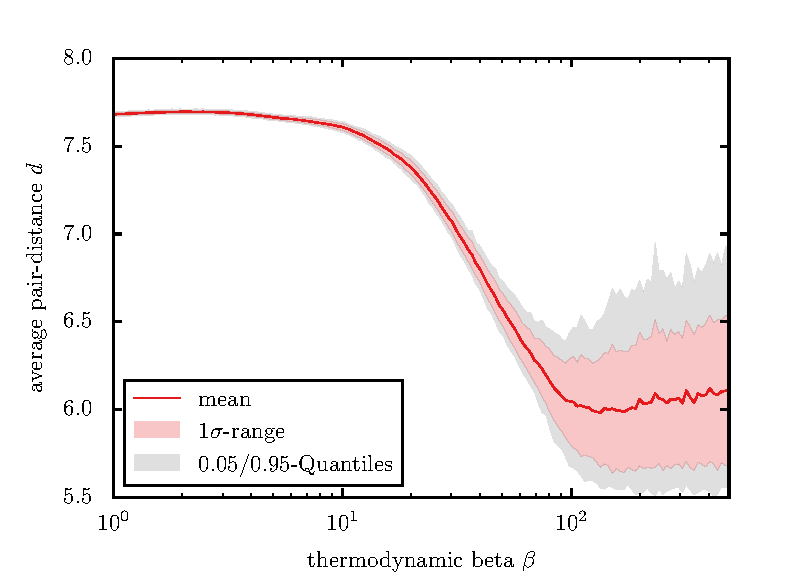
\includegraphics{./figures/temp_dep_coulomb2d.pdf}
	\caption{Temperature dependence 2d case}
\end{figure}
\begin{figure}
	\centering
	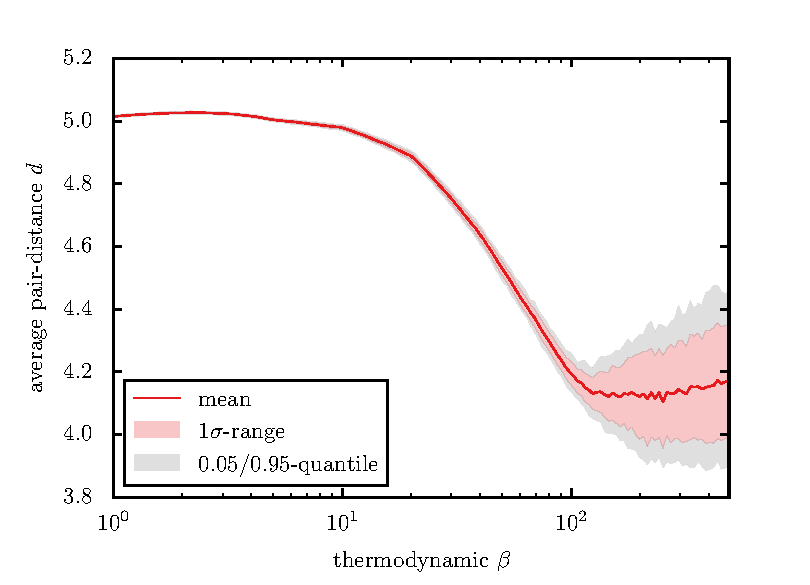
\includegraphics{./figures/temp_dep_coulomb3d.pdf}
	\caption{Temperature dependence 3d case}
\end{figure}


\subsection{Visualization} \label{sec:Visualisation}
3D Visualization?


\section{Further Analysis} \label{sec:Further_Analysis}



\FloatBarrier
% BIBLIOGRAPHY
\vspace{\fill}
\begin{thebibliography}{9}
\bibitem{schwabl}
	F. Schwabl,
	\emph{Statistische Mechanik},
	Springer, Berlin, 3rd edition 2006.
\end{thebibliography}

\begin{appendix}
	\newpage
	\section{Source code}
	The full source code can be found on \url{https://github.com/chrisieh/piap} (a \texttt{C++14} compliant compiler is needed).
	\subsection{CanonicalEnsemble{.}h} \label{sec:canonical_ensemble_source}
	\lstinputlisting[language=C++]{../code/src/CanonicalEnsemble.h}
\end{appendix}

\end{document}